\contribution{Landscape}
\shortcontributor{CS6230 : CAD for VLSI Project Report}
\shortcontribution{Overview}
\headnum{1}
\begin{paper}
\renewcommand*{\pagemark}{}

\section*{}
Domain Specific Hardware Accelerators are processors designed to perform a specialized task. These tasks extend from accelerators for signal processing to specific matrix multiplication cores concerning neural networks. These devices are power, area, and time optimized for a particular task and exploits parallelism, resulting in significant performance enhancement. Furthermore, these devices have Direct Memory Access, and sometimes these have an internal memory of capacity similar to the primary memory.
\section*{Overview\sdot}

\begin{figure}[H]
\centering
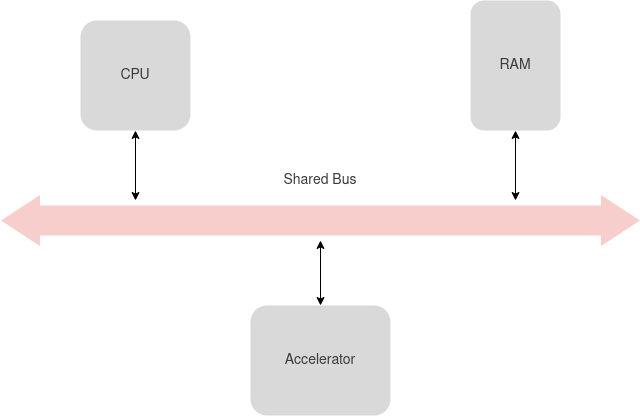
\includegraphics[width=8cm]{Images/Overview-Overview.png}
\caption{\content Overview of the system.}
\end{figure}
\nointend The principal objective of our project is to design vector accelerators for elementwise negation and statistics minima. These accelerators are connected to a common bus and have directory access to the memory, further lessening the CPU workload. The CPU issues instructions to the accelerators, which comprises pointers to data in the memory. There is no direct data transfer between the CPU and the accelerators. The result of the vector computation is written back to the memory. The Control Status Registers in these accelerators let the CPU control and read status from them. Vector instructions on float32, int8, int16 & int32 data types are implemented. 
\section*{Parameterized and Modular Design\sdot}
Our design is completely modular. All the modules, i.e., the CPU, Memory, and Accelerators, are parameterized. All the modules can be instantiated with many different combinations of parameters, including wordlength, data length, and bus data \& address width subjected to logical constraints.

\section*{Testbench, Simulation and Custom Assembler\sdot}

To ease the development process with better testing capabilities, we wrote a minimal assembler in Python that converts the sequences of instructions supported by our CPU into machine code, which can be utilized to initialize the instruction memory in Bluespec.\\
\begin{figure}[H]
\centering
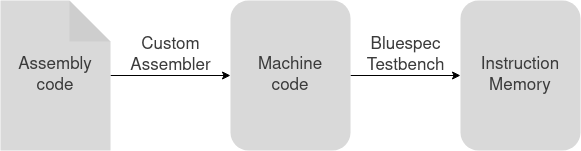
\includegraphics[width=8cm]{Images/Overview-Simulation.png}
\caption{\content Simulation of the system.}
\end{figure}
\noindent For more details about the instruction set, see section CPU.
\end{paper}